% Options for packages loaded elsewhere
\PassOptionsToPackage{unicode}{hyperref}
\PassOptionsToPackage{hyphens}{url}
\documentclass[
  ignorenonframetext,
  aspectratio=169,
]{beamer}
\newif\ifbibliography
\usepackage{pgfpages}
\setbeamertemplate{caption}[numbered]
\setbeamertemplate{caption label separator}{: }
\setbeamercolor{caption name}{fg=normal text.fg}
\beamertemplatenavigationsymbolsempty
% remove section numbering
\setbeamertemplate{part page}{
  \centering
  \begin{beamercolorbox}[sep=16pt,center]{part title}
    \usebeamerfont{part title}\insertpart\par
  \end{beamercolorbox}
}
\setbeamertemplate{section page}{
  \centering
  \begin{beamercolorbox}[sep=12pt,center]{section title}
    \usebeamerfont{section title}\insertsection\par
  \end{beamercolorbox}
}
\setbeamertemplate{subsection page}{
  \centering
  \begin{beamercolorbox}[sep=8pt,center]{subsection title}
    \usebeamerfont{subsection title}\insertsubsection\par
  \end{beamercolorbox}
}
% Prevent slide breaks in the middle of a paragraph
\widowpenalties 1 10000
\raggedbottom
\AtBeginPart{
  \frame{\partpage}
}
\AtBeginSection{
  \ifbibliography
  \else
    \frame{\sectionpage}
  \fi
}
\AtBeginSubsection{
  \frame{\subsectionpage}
}
\usepackage{iftex}
\ifPDFTeX
  \usepackage[T1]{fontenc}
  \usepackage[utf8]{inputenc}
  \usepackage{textcomp} % provide euro and other symbols
\else % if luatex or xetex
  \usepackage{unicode-math} % this also loads fontspec
  \defaultfontfeatures{Scale=MatchLowercase}
  \defaultfontfeatures[\rmfamily]{Ligatures=TeX,Scale=1}
\fi
\usepackage{lmodern}
\ifPDFTeX\else
  % xetex/luatex font selection
\fi
% Use upquote if available, for straight quotes in verbatim environments
\IfFileExists{upquote.sty}{\usepackage{upquote}}{}
\IfFileExists{microtype.sty}{% use microtype if available
  \usepackage[]{microtype}
  \UseMicrotypeSet[protrusion]{basicmath} % disable protrusion for tt fonts
}{}
\makeatletter
\@ifundefined{KOMAClassName}{% if non-KOMA class
  \IfFileExists{parskip.sty}{%
    \usepackage{parskip}
  }{% else
    \setlength{\parindent}{0pt}
    \setlength{\parskip}{6pt plus 2pt minus 1pt}}
}{% if KOMA class
  \KOMAoptions{parskip=half}}
\makeatother
\usepackage{longtable,booktabs,array}
\usepackage{caption}
\captionsetup[table]{skip=6pt}
\newcounter{none} % for unnumbered tables
\usepackage{calc} % for calculating minipage widths
\usepackage{caption}
% Make caption package work with longtable
\makeatletter
\def\fnum@table{\tablename~\thetable}
\makeatother
\usepackage{graphicx}
\makeatletter
\newsavebox\pandoc@box
\newcommand*\pandocbounded[1]{% scales image to fit in text height/width
  \sbox\pandoc@box{#1}%
  \Gscale@div\@tempa{\textheight}{\dimexpr\ht\pandoc@box+\dp\pandoc@box\relax}%
  \Gscale@div\@tempb{\linewidth}{\wd\pandoc@box}%
  \ifdim\@tempb\p@<\@tempa\p@\let\@tempa\@tempb\fi% select the smaller of both
  \ifdim\@tempa\p@<\p@\scalebox{\@tempa}{\usebox\pandoc@box}%
  \else\usebox{\pandoc@box}%
  \fi%
}
% Set default figure placement to htbp
\def\fps@figure{htbp}
\makeatother
\setlength{\emergencystretch}{3em} % prevent overfull lines
\providecommand{\tightlist}{%
  \setlength{\itemsep}{0pt}\setlength{\parskip}{0pt}}
% Auto-generated by infrastructure/rendering/_pdf_latex_helpers.py::extract_math_font_preamble.
% Minimal header passed to Pandoc via -H so Beamer slides pick up the same math font
% as the combined-PDF path. Adjust the manuscript's preamble.md to change the font globally.
\usepackage{unicode-math}
\setmathfont{latinmodern-math.otf}

% Manuscript macro/package fallbacks (newcommand -> providecommand).
% Core mathematics
\usepackage{amsmath}
\usepackage{amssymb}
% Document layout
% Tables
\usepackage{booktabs}
% Caption styling (booktabs already loaded above). Small caption font with a
% bold label ("Figure 1", "Table 2") gives the math/figure-heavy layout a
% consistent, journal-like caption rhythm without fighting pandoc-crossref —
% pandoc emits standard \caption{}, and caption/captionsetup only restyle it.
% ── Theorem environments ─────────────────────────────────────────────────
% amsthm is loaded above. The FedGVI<->Friston bridge is stated as a small
% number of theorems/definitions/lemmas/propositions/corollaries; sharing one
% counter (definition/lemma/proposition/corollary all step the `theorem`
% counter) gives a single monotone numbering 1, 2, 3, ... across all kinds, so
% authors can reference them as Theorem 1, Definition 2, Corollary 3 without a
% per-kind counter drifting out of order. Plain style for theorem-like results,
% definition style (upright body) for definitions.
% (algorithm2e intentionally not loaded: this manuscript states results as
% numbered amsthm Theorems/Definitions, not algorithm2e pseudocode.)
% Code listings
\usepackage{listings}
% Typography and formatting
% (siunitx intentionally not loaded: no \SI/\num units appear in this manuscript.)
% Cross-references and citations
% (cleveref and titlesec intentionally not loaded: unavailable in this TeX tree
% and not required. Cross-references resolve through pandoc-crossref's own
% \ref-style names — no \cref appears — and section heading styling falls back
% to the pandoc/LaTeX defaults.)
% ── TeX Live Basic-compatible mono font for code listings ────────────
% Latin Modern Mono is bundled with TeX Live Basic and keeps the manuscript
% renderable on minimal TeX installations. Mathematical Unicode coverage is
% provided separately by Latin Modern Math below, so the code font does not
% need a private JuliaMono installation.
%
% Use the TeX font filename rather than the system-family name: the minimal
% TeX Live fontconfig database may not register the OpenType family even though
% kpsewhich can resolve the bundled files.
% Math font for unicode-math: Latin Modern Math (TeX Live) has full BMP
% coverage including U+2223 (\mid), U+226A/226B (\ll/\gg), and the Greek/
% blackboard letters used in equations. Without an explicit \setmathfont,
% unicode-math falls back to lmroman text font which lacks several glyphs
% and emits "Missing character" warnings on every \mid in math mode.

% Slide layout defaults for warning-clean scientific decks.
\usepackage{etoolbox}
\IfFileExists{xurl.sty}{\usepackage{xurl}}{}
\IfFileExists{seqsplit.sty}{\usepackage{seqsplit}}{\newcommand{\seqsplit}[1]{#1}}
\protected\def\breakseq#1{\seqsplit{#1}}
\protected\def\breaktt#1{\begingroup\ttfamily\seqsplit{#1}\endgroup}
\setlength{\emergencystretch}{6em}
\tolerance=5000
\hbadness=10000
\hfuzz=1pt
\setlength{\tabcolsep}{2pt}
\AtBeginEnvironment{longtable}{\tiny\renewcommand{\arraystretch}{0.86}\setlength{\tabcolsep}{1pt}}
\AtBeginEnvironment{tabular}{\tiny\renewcommand{\arraystretch}{0.86}\setlength{\tabcolsep}{1pt}}
\AtBeginEnvironment{equation}{\tiny}
\AtBeginEnvironment{equation*}{\tiny}
\AtBeginEnvironment{align}{\tiny}
\AtBeginEnvironment{align*}{\tiny}
\AtBeginEnvironment{itemize}{\footnotesize}
\AtBeginEnvironment{enumerate}{\footnotesize}
\AtBeginEnvironment{description}{\footnotesize}
\setbeamerfont{caption}{size=\tiny}
\setbeamerfont{caption name}{size=\tiny}
\setbeamerfont{normal text}{size=\small}
\setbeamerfont{frametitle}{size=\small}
\setbeamerfont{section title}{size=\footnotesize}
\setbeamerfont{subsection title}{size=\footnotesize}
\setbeamertemplate{section page}{%
  \centering
  \begin{beamercolorbox}[sep=12pt,center,wd=\paperwidth]{section title}
    \parbox{0.86\paperwidth}{\centering\usebeamerfont{section title}\insertsection\par}
  \end{beamercolorbox}
}
\setbeamertemplate{subsection page}{%
  \centering
  \begin{beamercolorbox}[sep=8pt,center,wd=\paperwidth]{subsection title}
    \parbox{0.86\paperwidth}{\centering\usebeamerfont{subsection title}\insertsubsection\par}
  \end{beamercolorbox}
}
\setlength{\abovecaptionskip}{2pt}
\setlength{\belowcaptionskip}{0pt}

% Natbib and cross-reference fallbacks — slides don't load natbib
% or cleveref, but combined-PDF manuscript prose may emit these
% commands. The fallback renders citations as a bracketed key list
% and cross-references as detokenized labels so slides don't fail on
% undefined control sequences or raw underscores. \providecommand is
% a no-op if packages load later.
\providecommand{\citep}[1]{[#1]}
\providecommand{\citet}[1]{#1}
\providecommand{\citealp}[1]{#1}
\providecommand{\citeauthor}[1]{#1}
\providecommand{\citeyear}[1]{#1}
\providecommand{\cref}[1]{\texttt{\detokenize{#1}}}
\providecommand{\Cref}[1]{\texttt{\detokenize{#1}}}
\providecommand{\crefrange}[2]{\texttt{\detokenize{#1}}--\texttt{\detokenize{#2}}}
\providecommand{\Crefrange}[2]{\texttt{\detokenize{#1}}--\texttt{\detokenize{#2}}}
\providecommand{\paragraph}[1]{\textbf{#1}\ }

% Opt-in accessible presentation profile.
\setbeamerfont{normal text}{size*={20pt}{24pt}}
\setbeamerfont{frametitle}{size*={28pt}{32pt}}
\setbeamerfont{section title}{size*={28pt}{32pt}}
\setbeamerfont{subsection title}{size*={28pt}{32pt}}
\setbeamerfont{caption}{size*={16pt}{19pt}}
\setbeamerfont{caption name}{size*={16pt}{19pt}}
\setbeamerfont{itemize/enumerate body}{size*={20pt}{24pt}}
\setbeamerfont{itemize/enumerate subbody}{size*={20pt}{24pt}}
\setbeamerfont{itemize/enumerate subsubbody}{size*={20pt}{24pt}}
\setbeamerfont{itemize item}{size*={20pt}{24pt}}
\setbeamerfont{itemize subitem}{size*={20pt}{24pt}}
\setbeamerfont{itemize subsubitem}{size*={20pt}{24pt}}
\setbeamerfont{description body}{size*={20pt}{24pt}}
\setbeamerfont{description item}{size*={20pt}{24pt}}
\setbeamerfont{quote}{size*={20pt}{24pt}}
\setbeamerfont{quotation}{size*={20pt}{24pt}}
\AtBeginEnvironment{longtable}{\fontsize{20pt}{24pt}\selectfont}
\AtBeginEnvironment{tabular}{\fontsize{20pt}{24pt}\selectfont}
\AtBeginEnvironment{equation}{\fontsize{20pt}{24pt}\selectfont}
\AtBeginEnvironment{equation*}{\fontsize{20pt}{24pt}\selectfont}
\AtBeginEnvironment{align}{\fontsize{20pt}{24pt}\selectfont}
\AtBeginEnvironment{align*}{\fontsize{20pt}{24pt}\selectfont}
\AtBeginEnvironment{itemize}{\fontsize{20pt}{24pt}\selectfont}
\AtBeginEnvironment{enumerate}{\fontsize{20pt}{24pt}\selectfont}
\AtBeginEnvironment{description}{\fontsize{20pt}{24pt}\selectfont}
\AtBeginDocument{\usebeamerfont{normal text}}
\newlength{\AFSlideTableWidth}
% The fixed footer reservation is calibrated with the semantic seven-line regular-body budget.
\setbeamertemplate{footline}{%
  \leavevmode\vbox{%
    \hbox{%
      \begin{beamercolorbox}[wd=\paperwidth,ht=16pt,dp=3pt,center]{author in head/foot}%
        \fontsize{16pt}{19pt}\selectfont Untagged PDF derivative \textbar\ \href{../web/index.html}{HTML reader}%
      \end{beamercolorbox}%
    }%
    \vskip6pt%
  }%
}
% Accessible footer reserved height: 25pt.

\newtheorem{proposition}{Proposition}
\newtheorem{hypothesis}{Hypothesis}
\newtheorem{remark}[theorem]{Remark}
\newtheorem{axiom}{Axiom}
\newtheorem{property}{Property}
\usepackage{bookmark}
\IfFileExists{xurl.sty}{\usepackage{xurl}}{} % add URL line breaks if available
\urlstyle{same}
% fallback for those not using the hyperref driver hyperxmp:
\makeatletter
\@ifundefined{xmpquote}{\newcommand{\xmpquote}[1]{#1}}{}
\makeatother
\hypersetup{
  hidelinks,
  pdfcreator={LaTeX via pandoc}}

\author{\texorpdfstring{}{}}
\date{}

\begin{document}

\begin{frame}{Moving sentinel world: communication contrast depends on
field of view}
\protect\phantomsection\label{sec:results-moving}
The hidden-state/action relation for this extension is summarized in the
categorical loop schematic fig.~5; the results below
remain the executed moving-world comparisons,
\end{frame}

\begin{frame}{Moving sentinel world (part 2)}
not a claim that the schematic's full loop is present in every flat
belief-sharing study.
\end{frame}

\begin{frame}{Moving sentinel world (part 3)}
The static sentinel world lets every agent observe the same shared
latent, so belief sharing is a refinement rather than a requirement. To
stress the \emph{necessity} of communication we add movement and
\textbf{disjoint} fields of view.
\end{frame}

\begin{frame}{Moving sentinel world (part 4)}
The world is a linear grid of 4 cells holding a single binary threat ---
left half (state 0) or right half (state 1). The 2 sentinels start at
evenly tiled positions and each observe a half-open window of cells, so
in the default setup agent 0 watches the left half and agent 1 the right
half: their views do not overlap.
\end{frame}

\begin{frame}{Moving sentinel world (part 5)}
Each agent's likelihood is a confident, signed presence reading for the
half it can see, and three control paths (stay / left / right) let it
reposition. The expected-free-energy policy scores each candidate move
by the expected posterior entropy after one observation and takes the
most information-seeking step.
\end{frame}

\begin{frame}{Moving sentinel world (part 6)}
We run 960 trials of 6 steps each under three conditions:
\emph{isolated} (random moves, no sharing), \emph{communicating} (random
moves plus a log-linear-pool consensus each step), and \emph{EFE-guided}
(information-seeking moves plus the same sharing).
\end{frame}

\begin{frame}{Moving sentinel world (part 7)}
The measured consensus accuracies are 0.999 (isolated), 0.977
(communicating), and 0.978 (EFE-guided), with a communicating
free-energy gap of -0.528 nats relative to the isolated baseline
(negative:
\end{frame}

\begin{frame}{Moving sentinel world (part 8)}
no free-energy advantage over isolated in this binary-complement regime
of logically complete half-views) (fig.~26).
\end{frame}

\begin{frame}{Moving sentinel world (part 9)}
Across 128 independent seeds the EFE-guided accuracy is 0.983 (95 \% CI
0.982--0.984), the communicating (random-moves + sharing) accuracy is
0.982 (95 \% CI 0.982--0.983), and the isolated accuracy is 0.999 (95 \%
CI 0.999--0.999).
\end{frame}

\begin{frame}{Moving sentinel world (part 10)}
In this binary-complement regime the isolated condition is in fact
significantly \emph{higher} on accuracy than the EFE-guided sharing
condition --- their 95 \% intervals do not overlap --- and the
EFE-vs-isolated accuracy contrast yields Wilcoxon signed-rank
\(p = 9.27 \times 10^{-23}\) (significant; isolated higher),
\end{frame}

\begin{frame}{Moving sentinel world (part 11)}
effect size \(r = 1.000\) (large). Sharing is therefore not merely
unnecessary in this regime; it costs a small but reliable amount of
accuracy.
\end{frame}

\begin{frame}{Moving sentinel world (part 12)}
Nor does sharing lower free energy here: the EFE free-energy gap
(isolated surprise minus the EFE-guided condition's surprise) is -0.368
nats (95 \% CI -0.384---0.353) --- negative, so the pooled consensus is
slightly \emph{more} surprised by the true state than the isolated
baseline, because a single agent's view already suffices.
\end{frame}

\begin{frame}{Moving sentinel world (part 13)}
The accuracy case for \emph{necessity} is therefore made only in the
larger-state-space disjoint-FOV extension below, not by these
binary-complement numbers.
\end{frame}

\begin{frame}{Moving sentinel world (part 14)}
We report these numbers as measured, not assumed. The binary world
carries a logical complement: ruling out one's own half implies the
other, so a single agent's ``not detected'' still carries information
about the global state, and an isolated agent is not strictly blind.
\end{frame}

\begin{frame}{Moving sentinel world (part 15)}
By design, the intended \emph{cannot-decide-alone} regime is the
high-noise, few-step corner where one sensor's evidence cannot overcome
the flat prior; there belief sharing is meant to fuse the two
complementary views into a decisive consensus. That regime is not
separately measured here --- the construction,
\end{frame}

\begin{frame}{Moving sentinel world (part 16)}
the three actions, the EFE rule, and the exact condition protocol are
detailed in the supplement (sec.~14.8).
\end{frame}

\begin{frame}{Moving sentinel world (part 17)}
\begin{figure}
\centering
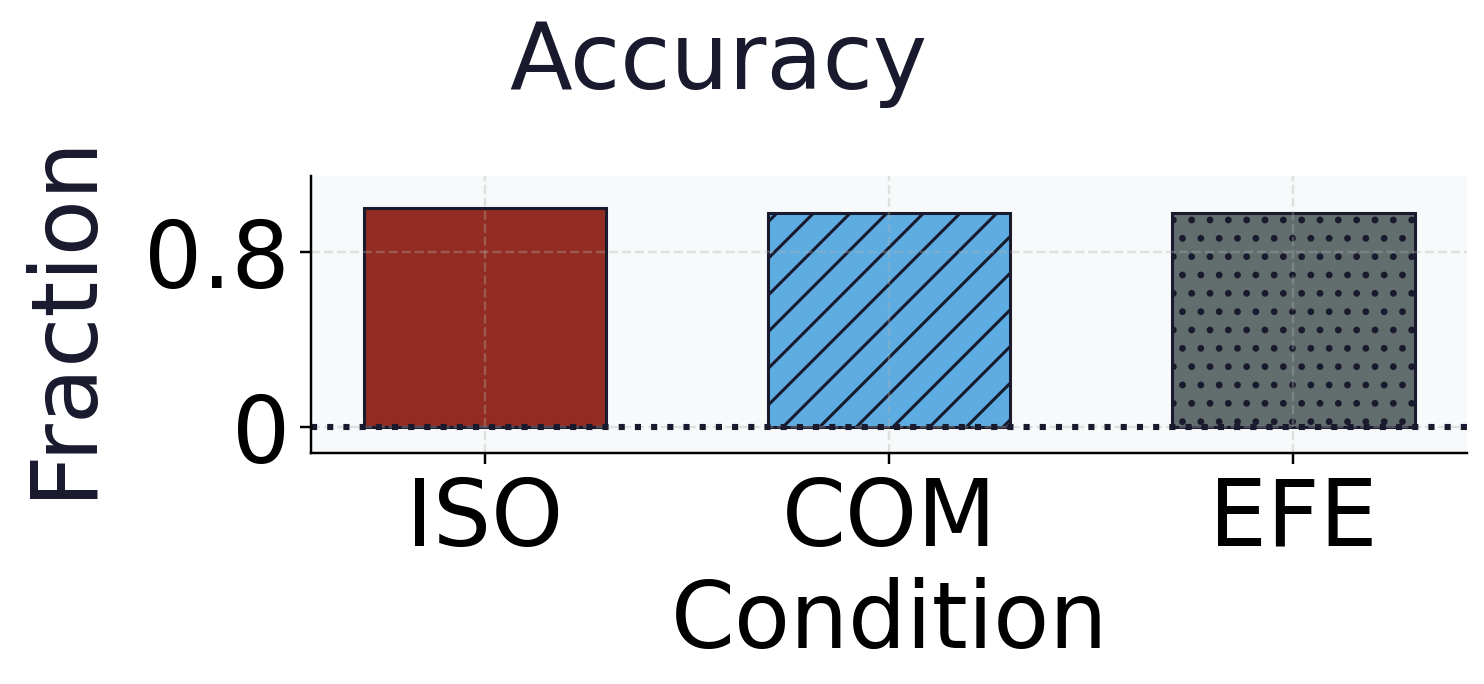
\includegraphics[keepaspectratio,width=0.98\linewidth,height=0.8\textheight,alt={Accuracy: all isolated, communicating and EFE-guided values in fraction, retaining signed values and ties.}]{../figures/moving_world.slide-accuracy.png}
\refstepcounter{figure}\label{fig:moving-world-slide-panel-1}
\end{figure}
\end{frame}

\begin{frame}{Moving sentinel world (part 18)}
\begin{figure}
\centering

\includegraphics[keepaspectratio,width=0.98\linewidth,height=0.8\textheight,alt={Accuracy (fraction): ISO +0.999; COM +0.9771; EFE +0.9781.}]{../figures/moving_world.slide-accuracy-values.png}
\refstepcounter{figure}\label{fig:moving-world-slide-panel-2}
\end{figure}
\end{frame}

\begin{frame}{Moving sentinel world (part 19)}
\begin{figure}
\centering
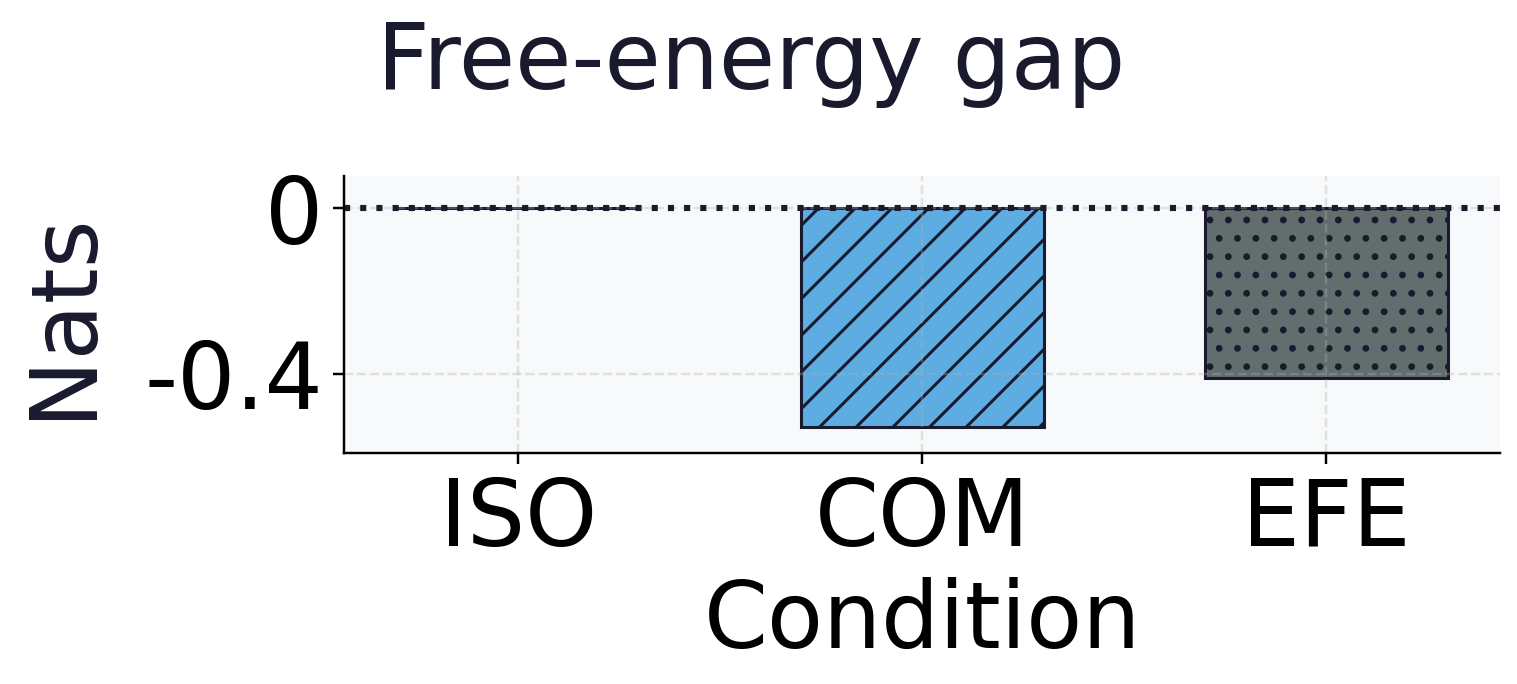
\includegraphics[keepaspectratio,width=0.98\linewidth,height=0.8\textheight,alt={Free-energy gap: all isolated, communicating and EFE-guided values in nats, retaining signed values and ties.}]{../figures/moving_world.slide-free-energy-gap.png}
\refstepcounter{figure}\label{fig:moving-world-slide-panel-3}
\end{figure}
\end{frame}

\begin{frame}{Moving sentinel world (part 20)}
\begin{figure}
\centering

\includegraphics[keepaspectratio,width=0.98\linewidth,height=0.8\textheight,alt={Free-energy gap (nats): ISO +0; COM -0.5285; EFE -0.4099.}]{../figures/moving_world.slide-free-energy-gap-values.png}
\refstepcounter{figure}\label{fig:moving-world-slide-panel-4}
\end{figure}
\end{frame}

\begin{frame}{Moving sentinel world (part 21)}
\begin{figure}
\centering
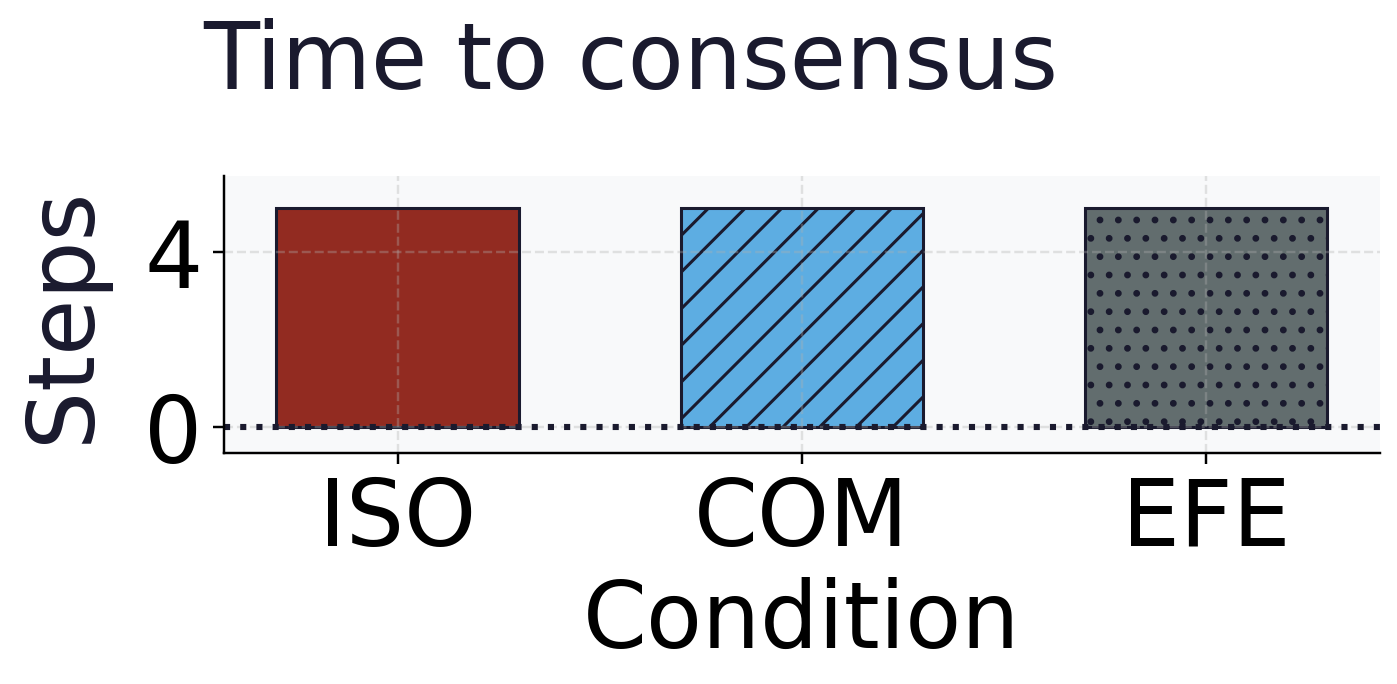
\includegraphics[keepaspectratio,width=0.98\linewidth,height=0.8\textheight,alt={Time to consensus: all isolated, communicating and EFE-guided values in steps, retaining signed values and ties.}]{../figures/moving_world.slide-n-steps-to-consensus.png}
\refstepcounter{figure}\label{fig:moving-world-slide-panel-5}
\end{figure}
\end{frame}

\begin{frame}{Moving sentinel world (part 22)}
\begin{figure}
\centering
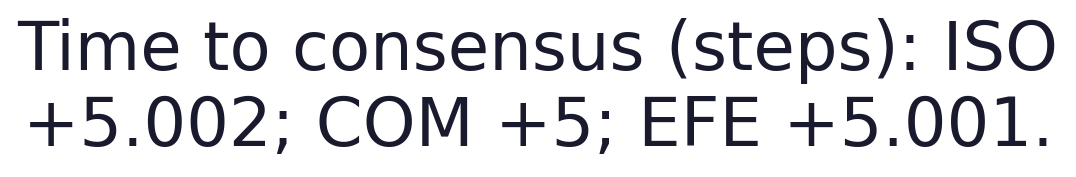
\includegraphics[keepaspectratio,width=0.98\linewidth,height=0.8\textheight,alt={Time to consensus (steps): ISO +5.002; COM +5; EFE +5.001.}]{../figures/moving_world.slide-n-steps-to-consensus-values.png}
\refstepcounter{figure}\label{fig:moving-world-slide-panel-6}
\end{figure}
\end{frame}

\begin{frame}{Moving sentinel world (part 23)}
\begin{figure}
\centering

\includegraphics[keepaspectratio,width=0.98\linewidth,height=0.8\textheight,alt={Accuracy gains over isolated: COM -0.022; EFE -0.021.}]{../figures/moving_world.slide-gains.png}
\refstepcounter{figure}\label{fig:moving-world-slide-panel-7}
\end{figure}
\end{frame}

\begin{frame}{Moving sentinel world (part 24)}
\begin{figure}
\centering
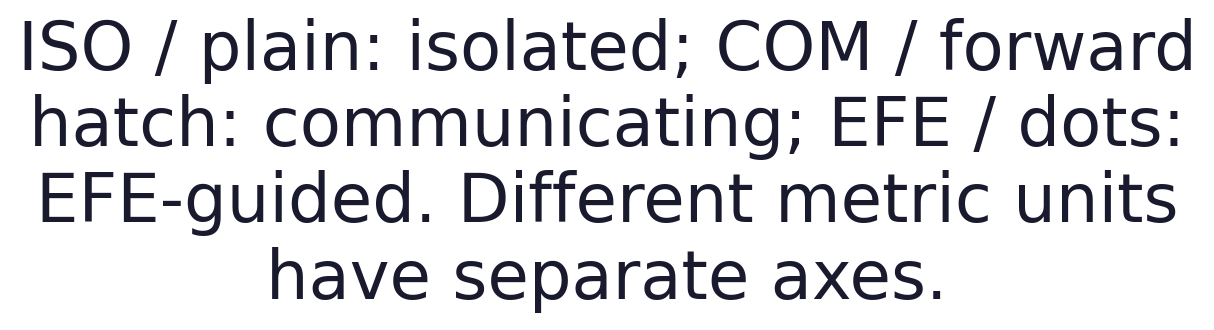
\includegraphics[keepaspectratio,width=0.98\linewidth,height=0.8\textheight,alt={ISO / plain: isolated; COM / forward hatch: communicating; EFE / dots: EFE-guided. Different metric units have separate axes.}]{../figures/moving_world.slide-key.png}
\refstepcounter{figure}\label{fig:moving-world-slide-panel-8}
\end{figure}
\end{frame}

\begin{frame}{Moving sentinel world (part 25)}
\begin{figure}
\centering
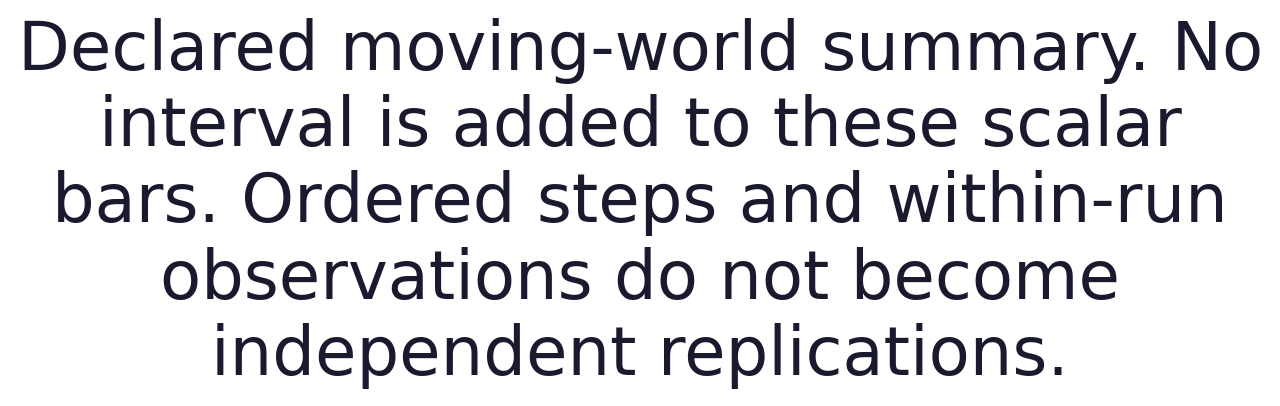
\includegraphics[keepaspectratio,width=0.98\linewidth,height=0.8\textheight,alt={Declared moving-world summary. No interval is added to these scalar bars. Ordered steps and within-run observations do not become independent replications.}]{../figures/moving_world.slide-scope.png}
\refstepcounter{figure}\label{fig:moving-world-slide-panel-9}
\end{figure}
\end{frame}

\begin{frame}{Disjoint field-of-view extension}
\protect\phantomsection\label{sec:results-disjoint-fov}
To test whether communication is necessary (not merely beneficial) when
observations are non-overlapping, we extend Study 5 to 3 agents each
observing a 2-position disjoint window of a 6-position state space
(chance-level accuracy 0.167).
\end{frame}

\begin{frame}{Disjoint field-of-view\ldots{} (part 2)}
Isolated agents achieve mean accuracy 0.35 --- above chance but far from
decisive, since no single agent can infer the global state from a
partial window alone. Communicating agents pool complementary beliefs to
reach 0.55 (gap 0.19).
\end{frame}

\begin{frame}{Disjoint field-of-view\ldots{} (part 3)}
This is now a powered result, not an illustrative point estimate. Across
128 independent seeds the isolated accuracy is 0.326 (95\% CI
0.320--0.332) and the communicating accuracy is 0.493 (95\% CI
0.487--0.499), both clearing the 0.167 chance baseline --- isolated
agents are \emph{not} at chance,
\end{frame}

\begin{frame}{Disjoint field-of-view\ldots{} (part 4)}
since a partial FOV plus majority voting still carries some signal.
\end{frame}

\begin{frame}{Disjoint field-of-view\ldots{} (part 5)}
The paired Wilcoxon signed-rank test (communicating vs.~isolated,
matched by seed) gives \(p = 9.35 \times 10^{-23}\), effect size
\(r = 1.000\) (large): communicating beats isolated on every one of the
128 seeds. This agreement saturates the rank-biserial effect at its
upper bound;
\end{frame}

\begin{frame}{Disjoint field-of-view\ldots{} (part 6)}
it does not turn the reported Wilcoxon signed-rank p-value into an exact
paired sign-test probability. The paired mean gap and its interval
quantify the accuracy contrast in its native units.
\end{frame}

\begin{frame}{Disjoint field-of-view\ldots{} (part 7)}
Given isolated performance is above chance, the precise claim is not
that communication is \emph{logically} necessary for any signal at all,
but that it is necessary to approach the communicating-level accuracy
under fully disjoint observations: the gap between the two conditions is
significant, large,
\end{frame}

\begin{frame}{Disjoint field-of-view\ldots{} (part 8)}
and reproducible, unlike the binary-complement contrast above.
\end{frame}

\begin{frame}{Disjoint field-of-view\ldots{} (part 9)}
We separately quantify EFE-guided navigation rather than asserting an
unquantified ``widens the gap'' effect. In a matched but smaller-scale
disjoint-FOV movement-policy comparison (2 agents, 4-position
binary-state grid, belief sharing active in both arms),
\end{frame}

\begin{frame}{Disjoint field-of-view\ldots{} (part 10)}
EFE-guided accuracy is 0.975 versus 0.977 for random movement
(\(p = 0.1046\), negligible effect). This comparison did not resolve an
accuracy difference in the configured near-ceiling regime with belief
sharing active; it does not establish equivalence of the movement
policies.
\end{frame}

\begin{frame}{Disjoint field-of-view\ldots{} (part 11)}
We report this as the null result it is rather than claiming an
unmeasured EFE benefit. fig.~27 summarizes the
necessity result.
\end{frame}

\begin{frame}{Disjoint field-of-view\ldots{} (part 12)}
\begin{figure}
\centering
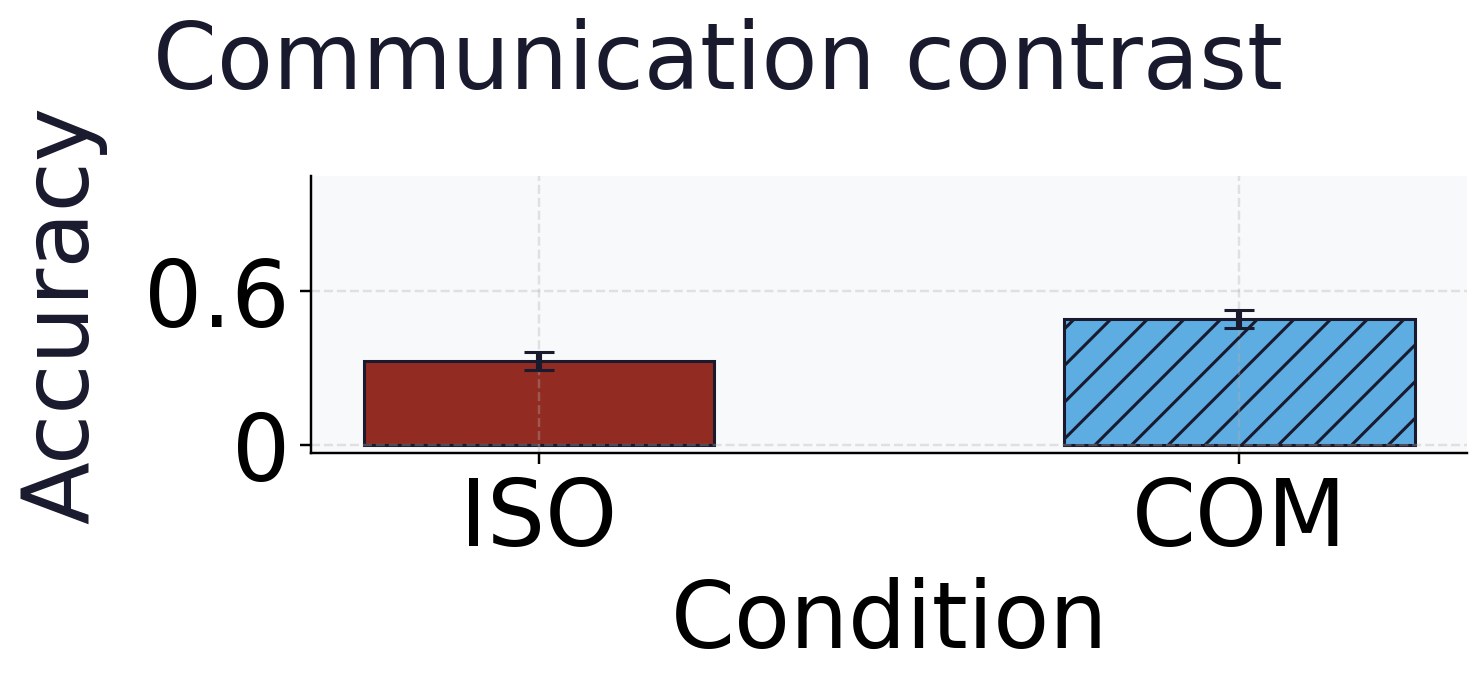
\includegraphics[keepaspectratio,width=0.98\linewidth,height=0.8\textheight,alt={communication: both condition means with seed standard-deviation whiskers on a common probability scale.}]{../figures/disjoint_fov_world.slide-communication.png}
\refstepcounter{figure}\label{fig:disjoint-fov-world-slide-panel-1}
\end{figure}
\end{frame}

\begin{frame}{Disjoint field-of-view\ldots{} (part 13)}
\begin{figure}
\centering
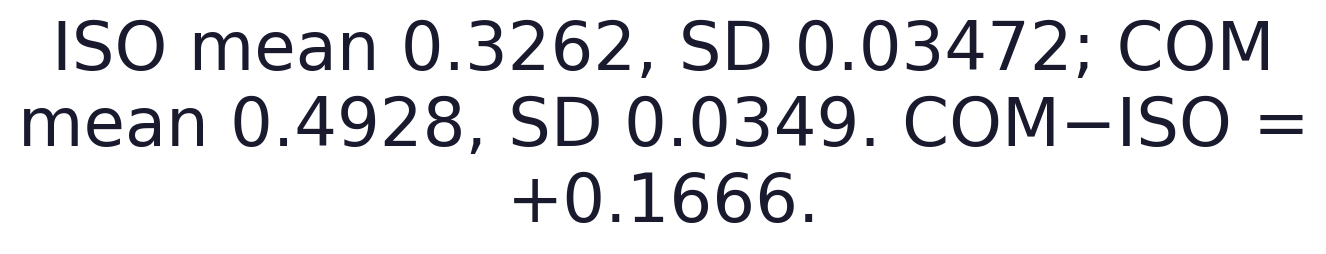
\includegraphics[keepaspectratio,width=0.98\linewidth,height=0.8\textheight,alt={ISO mean 0.3262, SD 0.03472; COM mean 0.4928, SD 0.0349. COM−ISO = +0.1666.}]{../figures/disjoint_fov_world.slide-communication-values.png}
\refstepcounter{figure}\label{fig:disjoint-fov-world-slide-panel-2}
\end{figure}
\end{frame}

\begin{frame}{Disjoint field-of-view\ldots{} (part 14)}
\begin{figure}
\centering
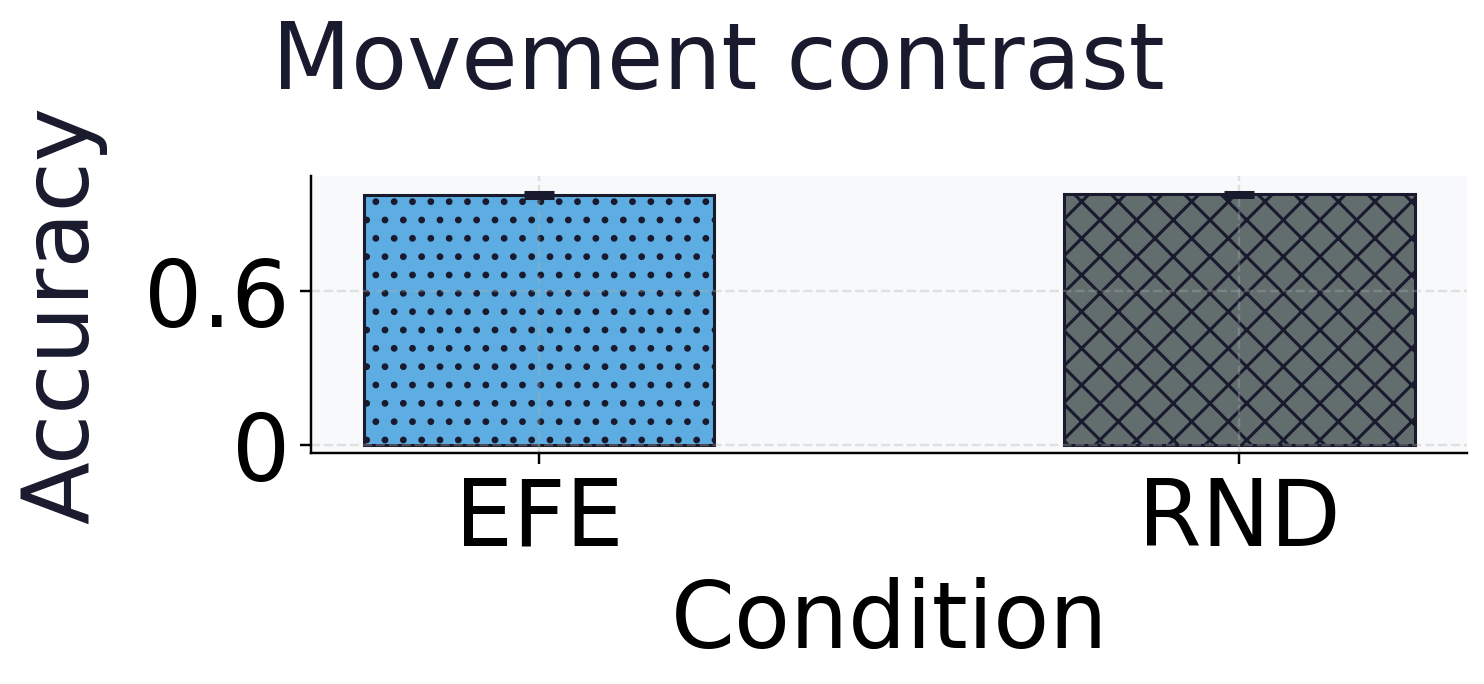
\includegraphics[keepaspectratio,width=0.98\linewidth,height=0.8\textheight,alt={movement: both condition means with seed standard-deviation whiskers on a common probability scale.}]{../figures/disjoint_fov_world.slide-movement.png}
\refstepcounter{figure}\label{fig:disjoint-fov-world-slide-panel-3}
\end{figure}
\end{frame}

\begin{frame}{Disjoint field-of-view\ldots{} (part 15)}
\begin{figure}
\centering
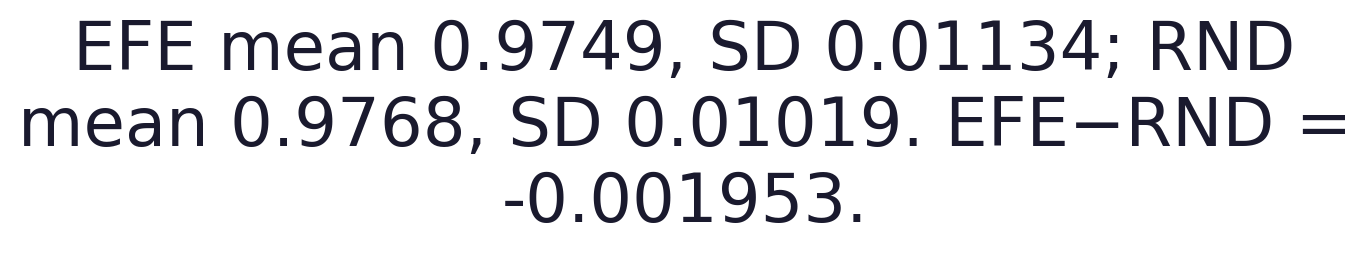
\includegraphics[keepaspectratio,width=0.98\linewidth,height=0.8\textheight,alt={EFE mean 0.9749, SD 0.01134; RND mean 0.9768, SD 0.01019. EFE−RND = -0.001953.}]{../figures/disjoint_fov_world.slide-movement-values.png}
\refstepcounter{figure}\label{fig:disjoint-fov-world-slide-panel-4}
\end{figure}
\end{frame}

\begin{frame}{Disjoint field-of-view\ldots{} (part 16)}
\begin{figure}
\centering

\includegraphics[keepaspectratio,width=0.98\linewidth,height=0.8\textheight,alt={ISO: isolated; COM: communicating; EFE: EFE-guided; RND: random movement. Hatches preserve condition identity.}]{../figures/disjoint_fov_world.slide-key.png}
\refstepcounter{figure}\label{fig:disjoint-fov-world-slide-panel-5}
\end{figure}
\end{frame}

\begin{frame}{Disjoint field-of-view\ldots{} (part 17)}
\begin{figure}
\centering
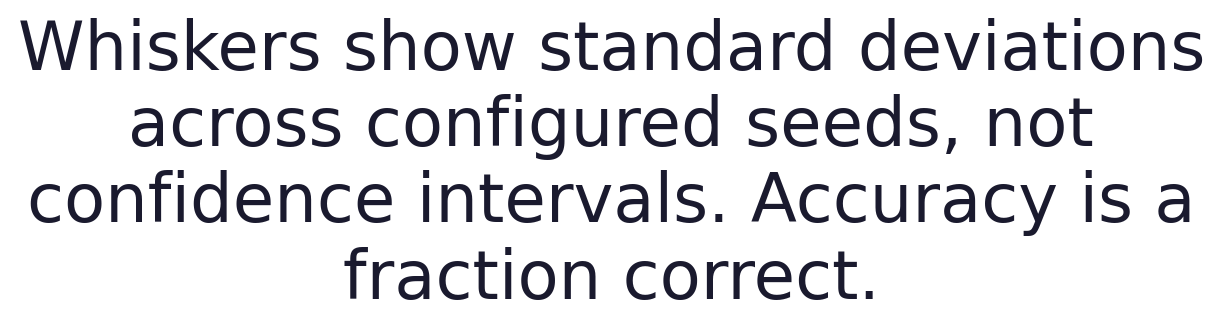
\includegraphics[keepaspectratio,width=0.98\linewidth,height=0.8\textheight,alt={Whiskers show standard deviations across configured seeds, not confidence intervals. Accuracy is a fraction correct.}]{../figures/disjoint_fov_world.slide-uncertainty.png}
\refstepcounter{figure}\label{fig:disjoint-fov-world-slide-panel-6}
\end{figure}
\end{frame}

\begin{frame}{Disjoint field-of-view\ldots{} (part 18)}
\begin{figure}
\centering
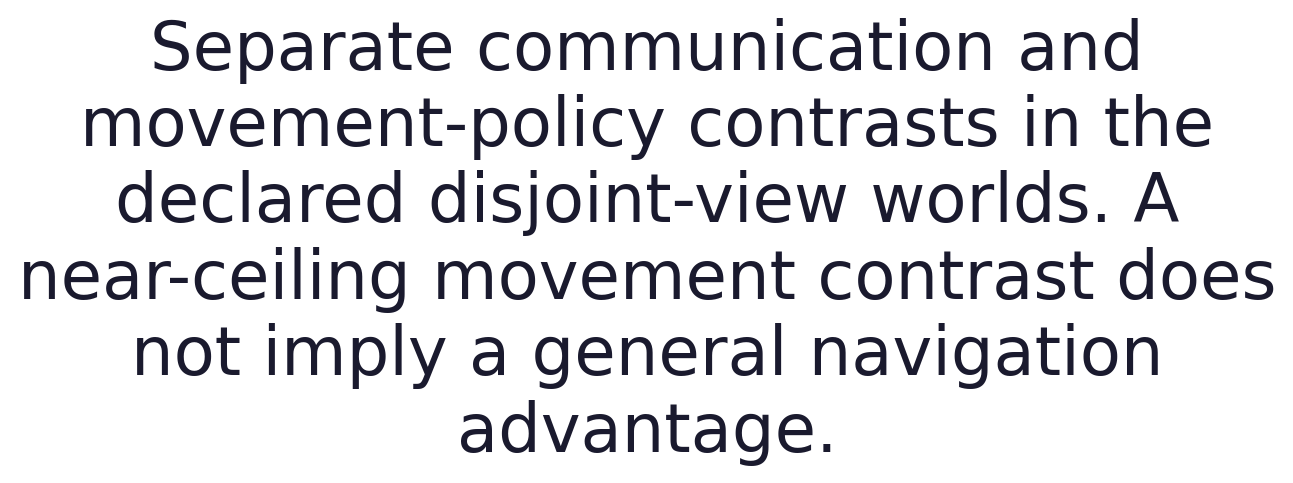
\includegraphics[keepaspectratio,width=0.98\linewidth,height=0.8\textheight,alt={Separate communication and movement-policy contrasts in the declared disjoint-view worlds. A near-ceiling movement contrast does not imply a general navigation advantage.}]{../figures/disjoint_fov_world.slide-scope.png}
\refstepcounter{figure}\label{fig:disjoint-fov-world-slide-panel-7}
\end{figure}
\end{frame}

\end{document}
